\chapter{Comportamiento longitudinal}
\label{ch:longitudinal-model}

El comportamiento longitudinal es un problema de regresión sobre cómo ha de comportarse la aceleración del \ac{dvu} en función de la información existente alrededor. El perfil de aceleración para el conjunto general de conductores tanto del conjunto de test como del de entrenamiento se ilustran en la figura~\ref{fig:acceleration-profiles}.

\begin{figure}
	\centering
	\subfloat[]{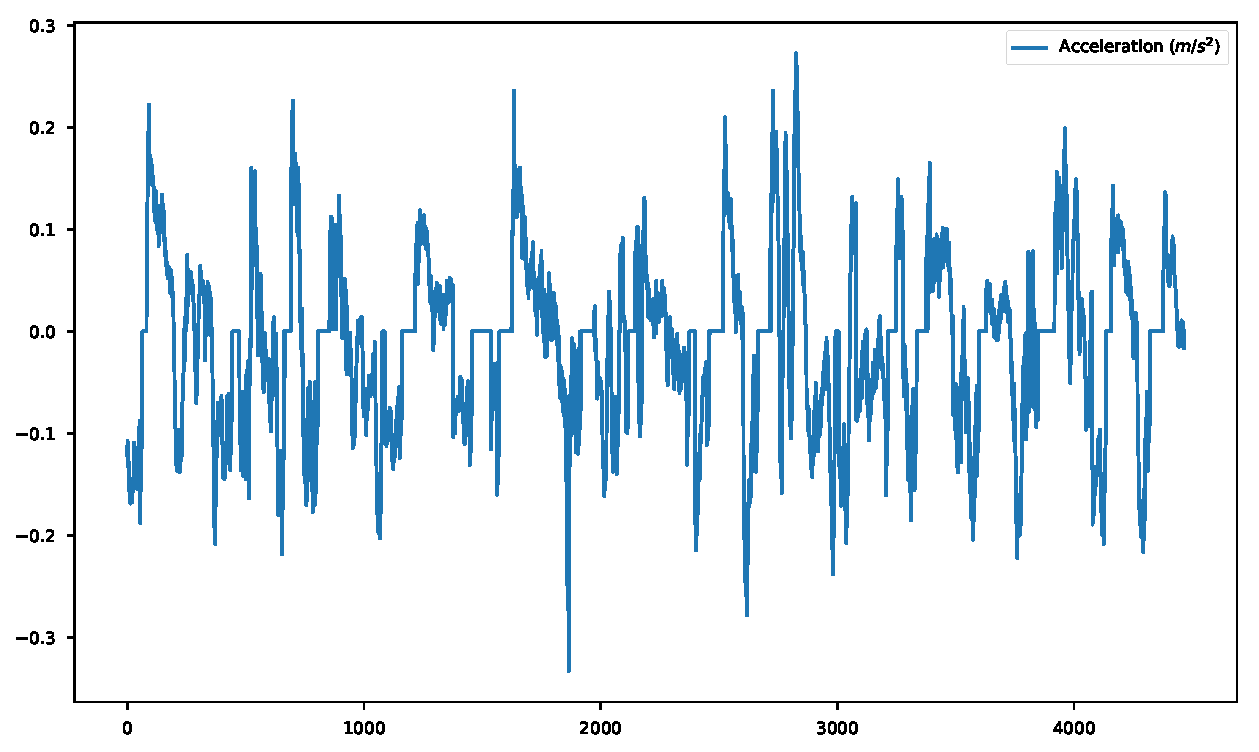
\includegraphics[width=.45\textwidth]{acceleration-profile-training}}\qquad
	\subfloat[]{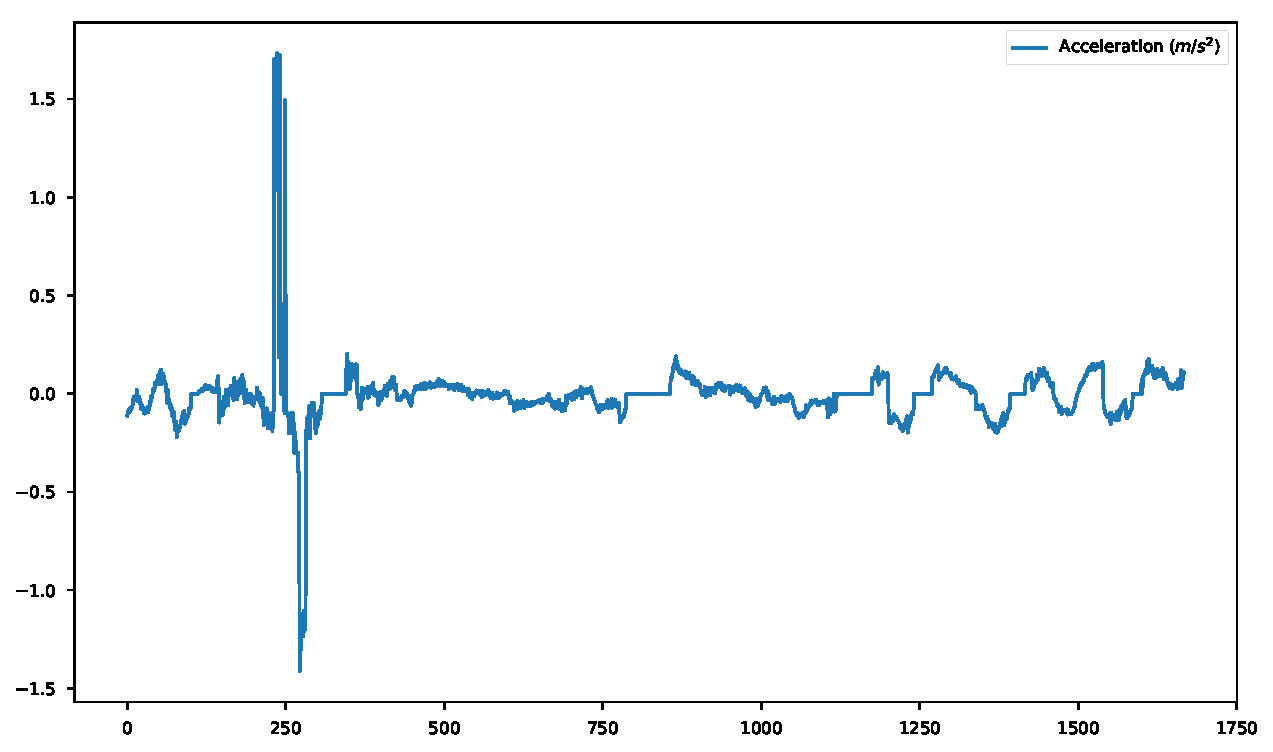
\includegraphics[width=.45\textwidth]{acceleration-profile-test}}
	\caption[Perfiles de aceleración a ajustar por los modelos. Conjuntos de entrenamiento y de test]{Perfiles de aceleración de los conjuntos de entrenamiento y test para ajustar por los modelos.}
	\label{fig:acceleration-profiles}
\end{figure}

Por la naturaleza del problema se han seleccionado dos técnicas diferentes para el ajuste del modelo:

\begin{enumerate}
	\item \ac{mlp}. Al ser un problema de regresión, el uso de \acp{mlp} en el comportamiento longitudinal está justificado a ser considerados éstos aproximadores universales~\cite{hornik1991approximation}\sidenote{El \textit{Teorema de aproximación Universal} postula que un \ac{mlp} con al menos una capa oculta es capaz de aproximar cualquier función si dispone de suficientes neuronas en ésta.}
	\item \ac{fcs}. La formulación de este problema se ajusta muy bien al funcionamiento de estos modelos, donde en función de las entradas y de acuerdo a una serie de reglas, el controlador toma una decisión para la salida. Además, los \ac{fcs} tienen la ventaja de que se puede explicar cómo funcionan, cosa que no es posible para un \ac{mlp} con una o más capas ocultas.
\end{enumerate}

Ambos modelos se entrenaran ajustando sus parámetros con un procedimiento basado en el descenso del gradiente denominado ADAM~\cite{kingma2014adam}. Su aplicación a los \ac{mlp} es directa, pero para \acp{fcs} es necesaria una representación que permita el uso de este método para su optimización. Esta representación es una de las aportaciones de esta tesis y se se explica en el apéndice \nameref{ch:fuzzy-controller-adjustment}.

\subsection{Descripción de los datasets}

Del conjunto de datos~\ref{tbl:main-variables} descrito en el capítulo~\nameref{ch:methodology} seleccionaremos aquellos indicadores de interés y generaremos un conjunto de entrenamiento y test para cada uno de los sujetos y un conjunto de entrenamiento y test para el total de conductores.

Dado que nuestros modelos se basan en un esquema \textit{feed-forward}, existe el inconveniente de que para ellos es imposible mantener una memoria del orden en el que se están sucediendo las entradas. Sin embargo, contamos con las derivadas de la posición respecto al líder y la velocidad (la aceleración y la velocidad al líder respectivamente), por lo consideramos que disponemos de información temporal suficiente para este problema en concreto.

\begin{table}
	\caption[Descripción de los conjuntos de datos]{Descripción de los conjuntos de datos para el entrenamiento de los modelos.}
	\label{tbl:cf-datasets-description}
	\begin{tabular}{ccccc}
		\toprule
		Nombre & Entradas & Salidas & Tamaño (training) & Tamaño (test) \\
		\midrule
		$CF_{S_1}$ & $7$ & $1$ & $1089$ & $543$ \\
		$CF_{S_2}$ & $7$ & $1$ & $1313$ & $560$ \\
		$CF_{S_3}$ & $7$ & $1$ & $2067$ & $668$ \\
		$CF_{S_A}$ & $7$ & $1$ & $4469$ & $1771$ \\
		\bottomrule
	\end{tabular}
\end{table}

\section{Modelo \ac{fcs}}

Se han realizado entrenamientos sobre arquitecturas con diferente número de particiones difusas en las variables. Las arquitecturas que se han considerado más relevantes (tras un proceso de ensayo y error con diferente número de particiones difusas) se describen en la tabla~\ref{tbl:cf-fcs-architectures}. 

\begin{table}
	\caption[Resumen de las arquitecturas \ac{fcs} para el modelo longitudinal]{Resumen de las arquitecturas de \ac{fcs} para el modelo longitudinal. La posición de cada número de la topología indica a qué variable lingüísticav se refiere (\textit{Distancia al líder}, Distancia a siguiente semáforo, Semáforo en verde, Semáforo en amarillo, Semáforo en rojo, Velocidad y velocidad de aproximación al líder respectivamente), siendo su valor el número de conjuntos difusos que configuran la partición difusa de la variable. Las arquitecturas seleccionadas en esta tabla son aquellas consideradas relevantes tras un proceso manual de ensayo y error.}
	\label{tbl:cf-fcs-architectures}
	\begin{tabular}{cccccc}
		\hline
		\multirow{2}{*}{Nombre} & \multirow{2}{*}{Arquitectura} & \multirow{2}{*}{Epochs} & \multicolumn{3}{c}{RMS}      \\ 
		&                            &                                          & Training & Validation & Test \\ \hline
		$FCS_1$ & $X, X, X$                 & $10^5$                  & $0.XXXXX$      & $0.XXXXX$        & $0.XXXXX$  \\
		$FCS_2$ & $X, X, X$               & $10^5$                  & $0.XXXXX$      & $0.XXXXX$        & $0.XXXXX$  \\
		$FCS_3$ & $X, X, X$              & $10^5$                  & $0.XXXXX$      & $0.XXXXX$        & $0.XXXXX$  \\
		$FCS_4$ & $X, X, X$          & $10^5$                  & $0.XXXXX$      & $0.XXXXX$        & $0.XXXXX$  \\ \hline
	\end{tabular}
\end{table}

Cada uno de los controladores se ha entrenado durante $250.000$ epochs. En la Figura~\ref{fig:adjusted-fcs} se puede observar la evolución en general y un detalle de la disminución del error en test de los controladores.

\begin{figure}
	\centering
	\subfloat[]{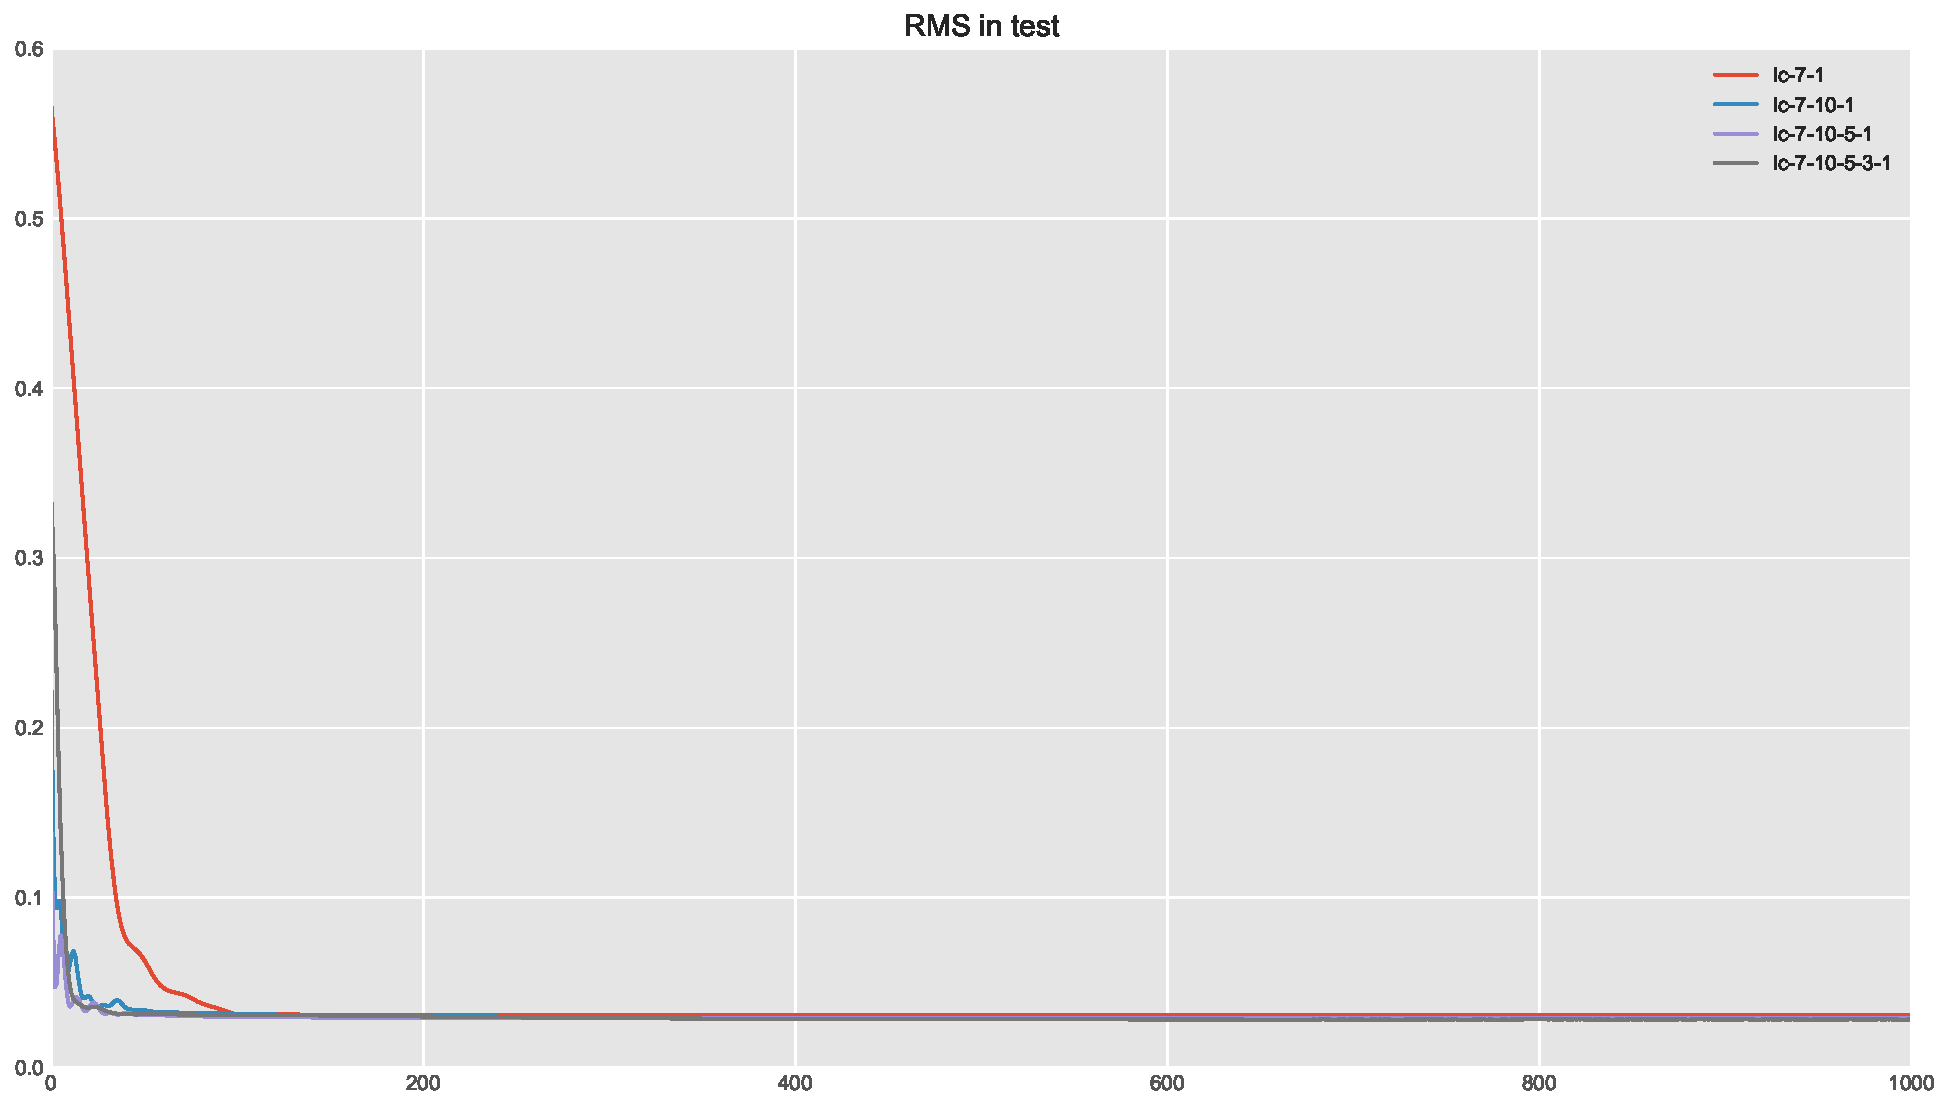
\includegraphics[width=.45\textwidth]{fcs-all-test}}\qquad
	\subfloat[]{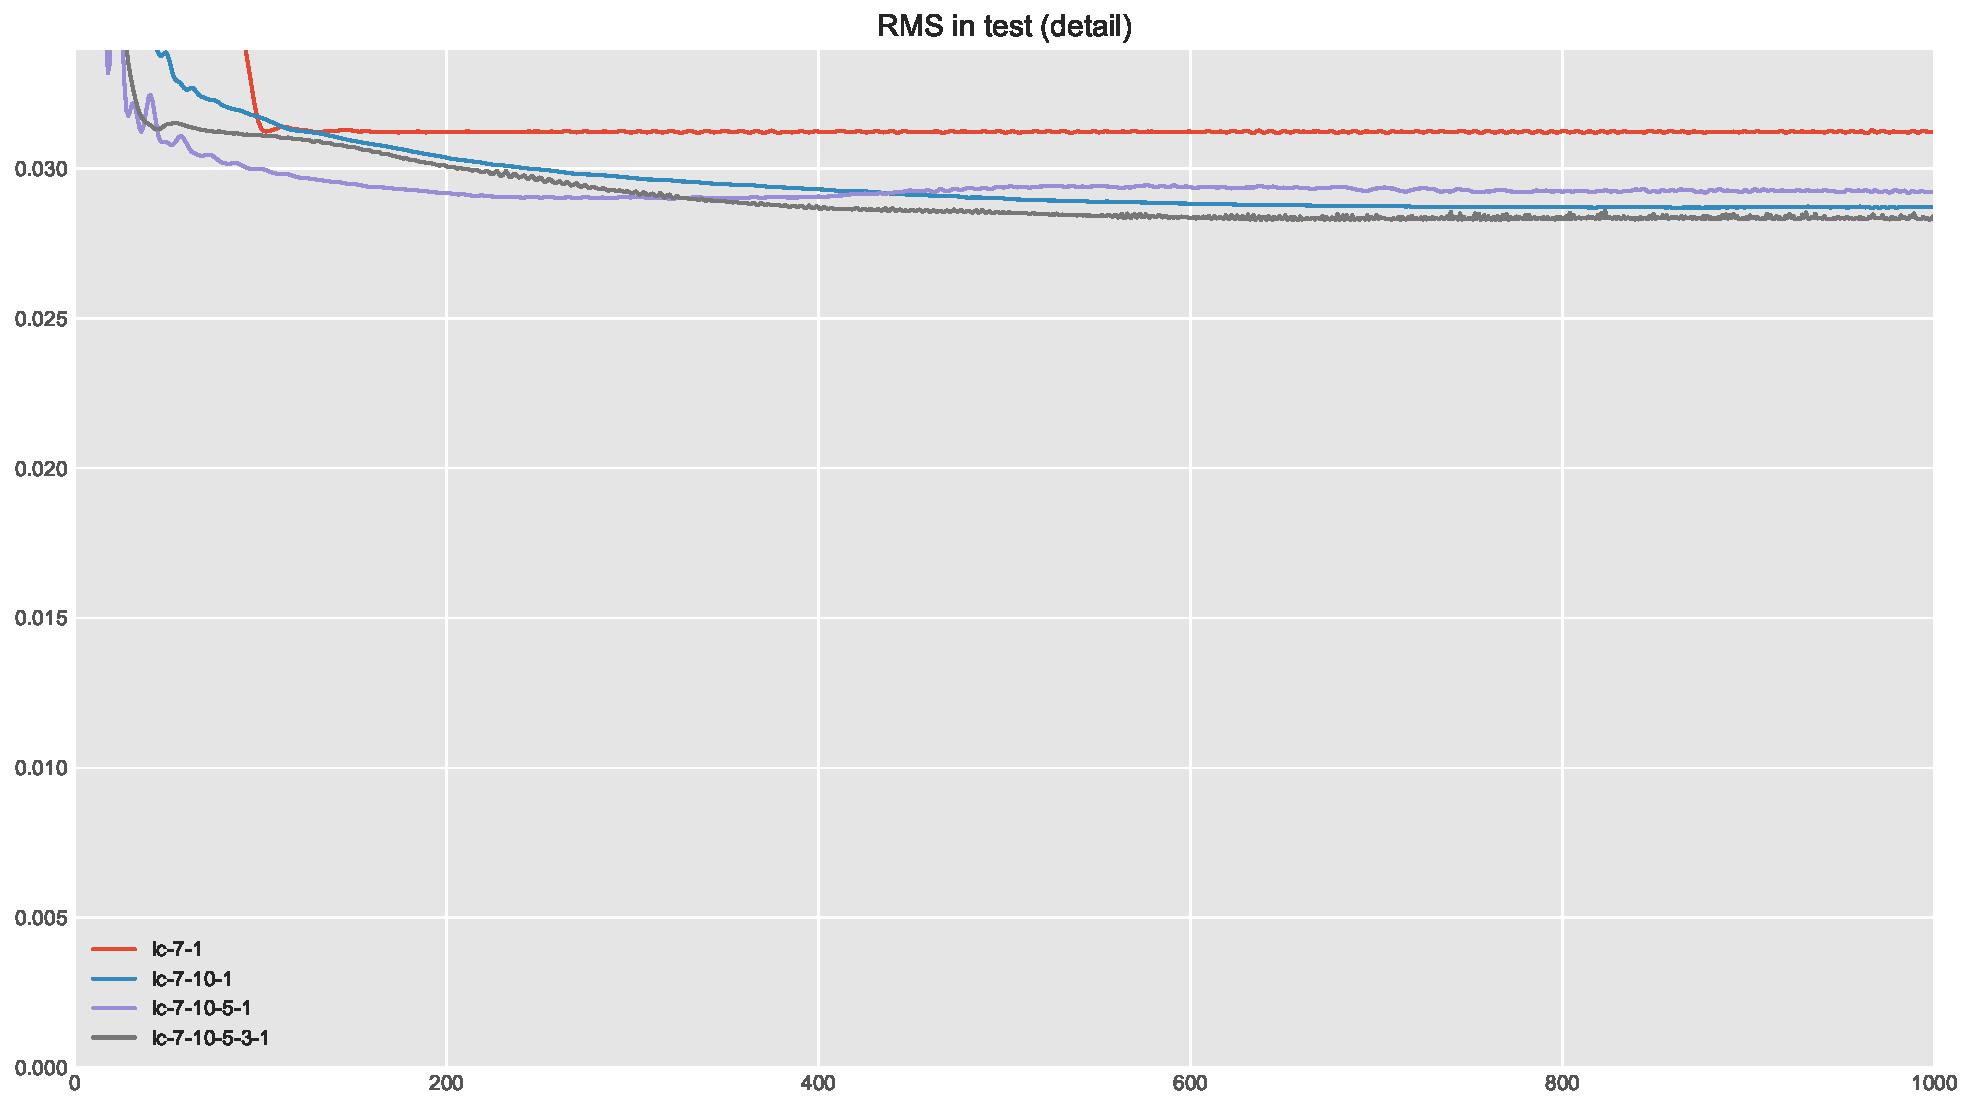
\includegraphics[width=.45\textwidth]{fcs-all-test-detail}}
	\caption[Evolución del error en test de los controladores difusos ajustados]{Visión general y detalle de la evolución del error en test de los diferentes controladores difusos ajustados.}
	\label{fig:adjusted-fcs}
\end{figure}

El proceso de entrenamiento seguido no ha sido el del ajuste de todas las variables en su conjunto. La razón principal de esto es que el ajuste de las variables que determinan las particiones difusas parece suceder órdenes de magnitud más rápido que el ajuste de los pesos asociados a las reglas.

Por tanto, y para este problema en concreto, El entrenamiento se realiza iterativamente alternando conjuntos de epochs dedicados a las reglas y conjuntos de epochs dedicados a las variables de las reglas difusas.

En lugar de eso se ha particionado el entrenamiento en secuencias sucesivas de entrenamiento de reglas y entrenamiento de particiones difusas. Concretamente, los $250.000$ epochs de entrenamiento se corresponden a $250$ iteraciones de $800$ epochs ajustando sólo las reglas seguidos de $200$ epochs ajustando las variables de las particiones difusas.

Empíricamente (y en este problema en concreto) se ha podido observar que el entrenamiento realizado de esta manera hace que el \ac{rmse} descienda más rápido en el mismo número de iteraciones.

Tras el entrenamiento, el controlador difuso que menor error en test arroja es el $FCS_2$\sidenote{
	Para el controlador $FCS_2$, la forma de sus particiones difusas queda, para las variables binarias sin apenas ajuste:
	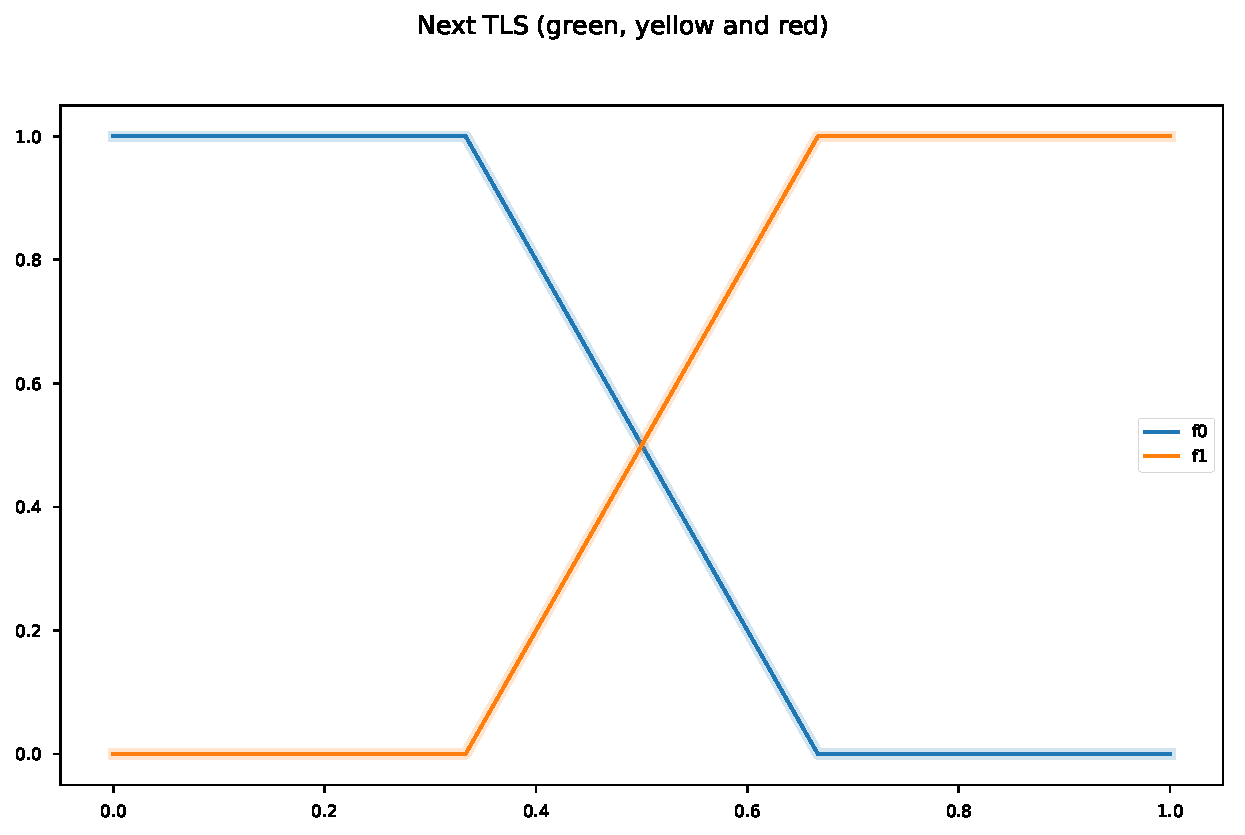
\includegraphics{fcs-best-architecture-next-tls-green-yellow-and-red-variable-partition}
	El resto de particiones sí se han visto modificadas:
	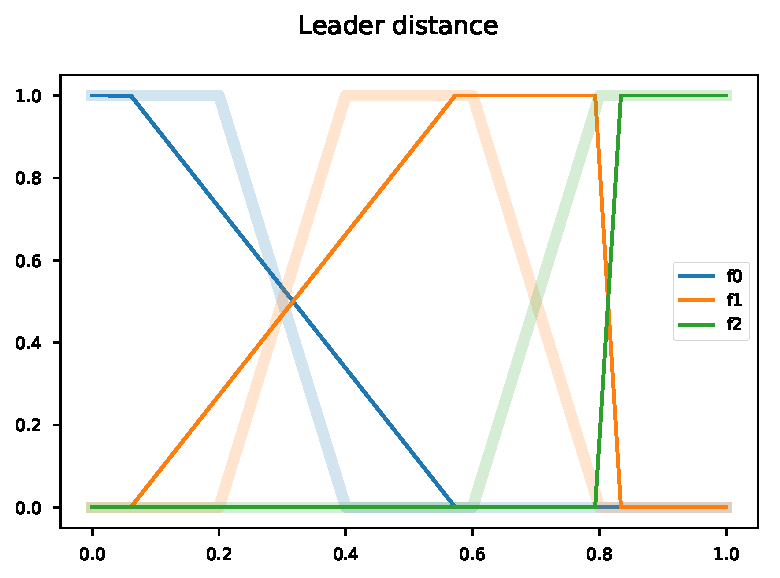
\includegraphics{fcs-best-architecture-leader-distance-variable-partition}
	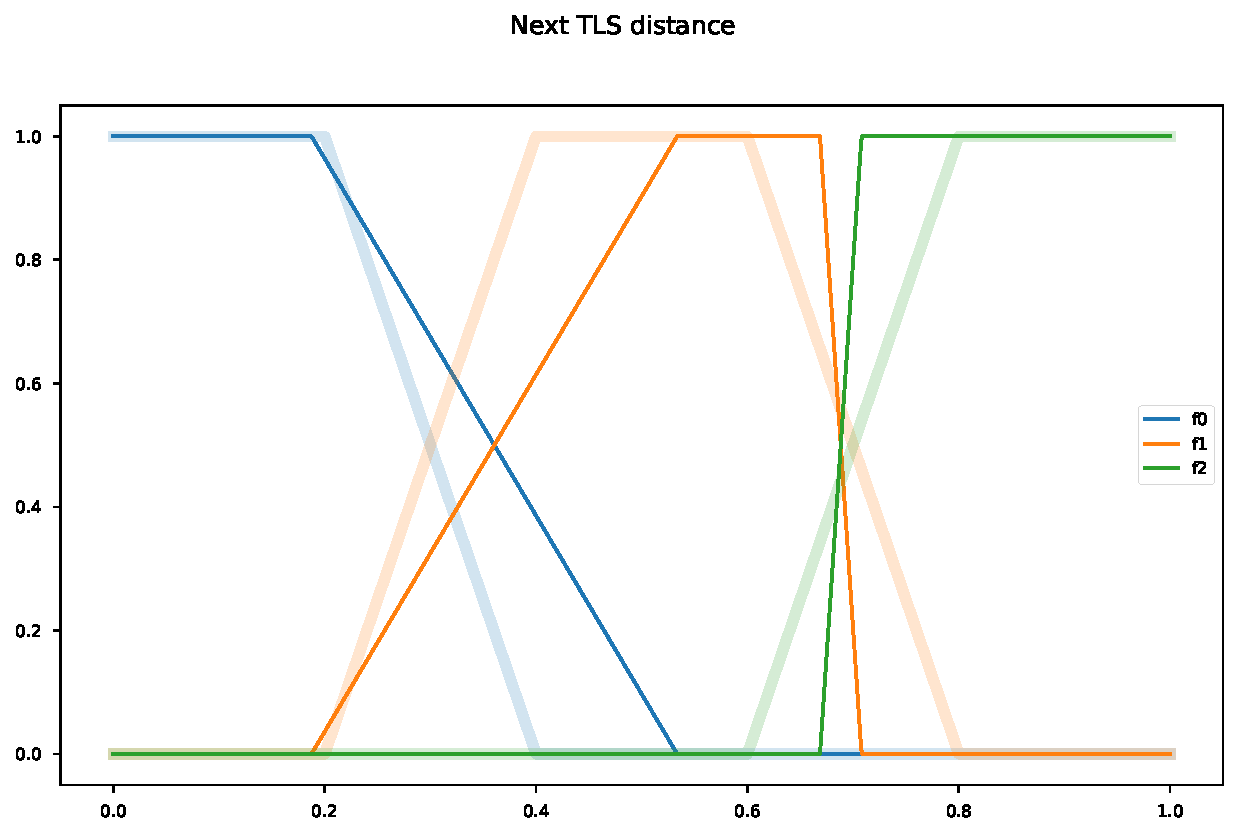
\includegraphics{fcs-best-architecture-next-tls-distance-variable-partition}
	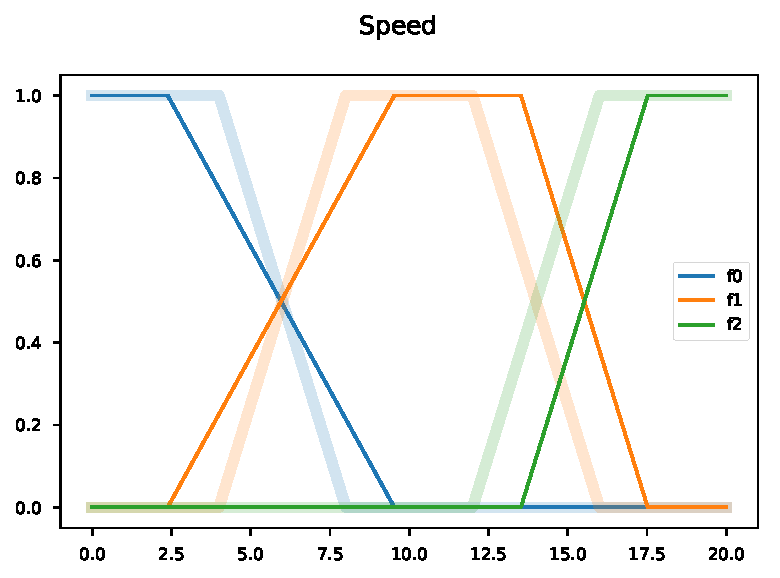
\includegraphics{fcs-best-architecture-speed-variable-partition}
	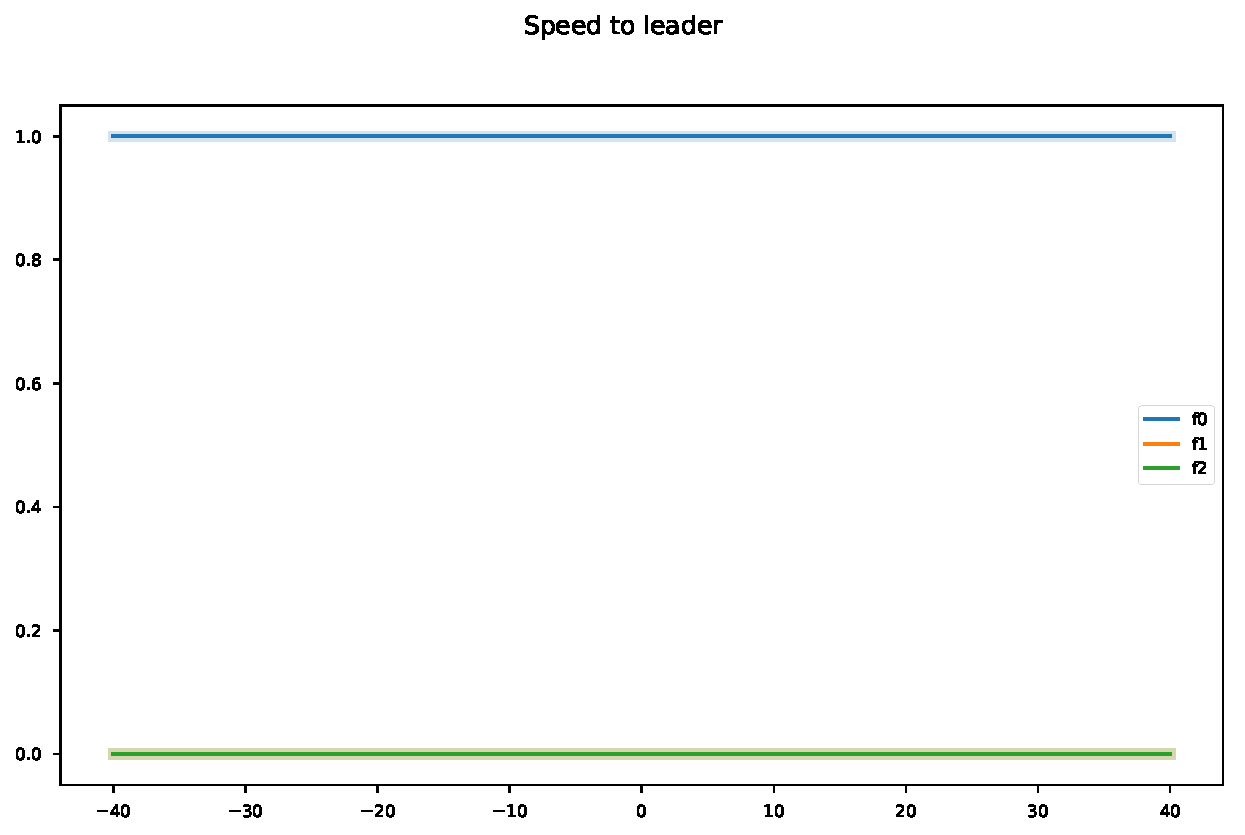
\includegraphics{fcs-best-architecture-speed-to-leader-variable-partition}
	En transparente se puede ver el estado inicial de la partición, y en opaco la forma de ésta tras el proceso de entrenamiento.
}. Por tanto, éste será el modelo seleccionado para la comparativa final.


\section{Modelo \ac{mlp}}

Para determinar el modelo óptimo de \ac{mlp} en comportamiento longitudinal, se han realizado entrenamientos sobre arquitecturas con diferente cantidad de neuronas y capas ocultas. Las arquitecturas más ilustrativas de todas las probadas se resumen en la tabla~\ref{tbl:cf-mlp-architectures}.

\begin{table*}
	\caption[Resumen de las arquitecturas \ac{mlp} para el modelo longitudinal]{Resumen de las arquitecturas de \ac{mlp} para el modelo longitudinal. La posición de cada número de la topología indica la capa, siendo su valor el número de nodos (neuronas) que incluye dicha capa. Las arquitecturas seleccionadas en esta tabla son aquellas consideradas relevantes tras un proceso manual de ensayo y error.}
	\label{tbl:cf-mlp-architectures}
	\begin{tabular}{ccccccc}
		\hline
		\multirow{2}{*}{Nombre} & \multirow{2}{*}{Topología} & \multirow{2}{*}{Epochs} & \multirow{2}{*}{Dropout} & \multicolumn{3}{c}{RMS}      \\
		&                            &                         &                          & Training & Validation & Test \\ \hline
		$MLP_1$ & $7, 16, 1$                 & $10^5$                  & $0.1$                    & $0.052741$      & $0.057301$        & $0.059253$  \\
		$MLP_2$ & $7, 8, 4, 1$               & $10^5$                  & $0.1$                    & $0.056341$      & $0.061951$        & $0.056607$  \\
		$MLP_3$ & $7, 16, 8, 1$              & $10^5$                  & $0.1$                    & $0.046404$      & $0.051878$        & $0.059681$  \\
		$MLP_4$ & $7, 16, 16, 8, 1$          & $10^5$                  & $0.1$                    & $0.042789$      & $0.046876$        & $0.060971$  \\ \hline
	\end{tabular}
\end{table*}

El modelo de neuronas de activación que se ha utilizado es de tipo tangente hiperbólica en todas las neuronas salvo en la última, que se ha utilizado una activación lineal en todas las neuronas salvo en la neurona de salida que se ha utilizado una activación lineal\sidenote{Se han utilizado también funciones de activación de tipo \ac{relu}, pero las tasas de error tras el entrenamiento eran notablemente más altas por lo que se ha optado al final por el uso de activación basada en tangente hiperbólica.}. Los pesos de la red han sido inicializados con una muestra aleatoria uniforme de valores reales en el intervalo $(-0.25, 0.25)$.

El error que se trata de minimizar es el error cuadrático medio entre los valores de aceleración del conjunto reales y los ajustados por el modelo. La Figura~\ref{fig:rms-all-in-training-and-validation-mlp-detail} muestra la evolución de este error durante el proceso de entrenamiento.

\begin{figure}
	\centering
	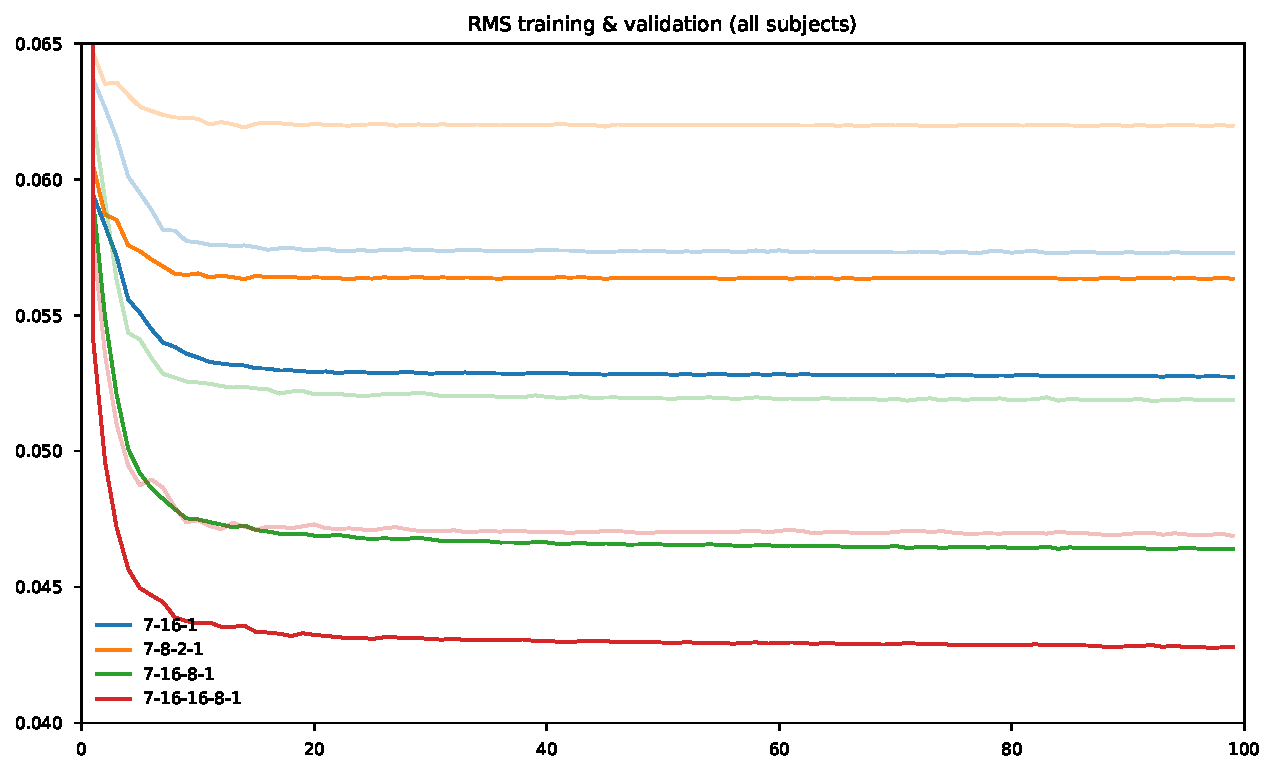
\includegraphics{rms-all-in-training-and-validation-mlp-detail}
	\caption[Evolución del error en entrenamiento en los \ac{mlp} para las arquitecturas seleccionadas]{Visión en detalle de la evolución del error en los conjuntos de entrenamiento y validación. Para cada arquitectura, el color más transparente se corresponde al error en el conjunto de validación..}
	\label{fig:rms-all-in-training-and-validation-mlp-detail}
\end{figure}

Estos errores se encuentran entre los \SI{0.05}{\metre\per\square\second} y los \SI{0.07}{\metre\per\square\second}, lo cual consideramos que es una aproximación aceptable. Una particularidad del problema ha sido la inestabilidad de los entrenamientos, esto es, la alta sensibilidad a los valores de inicialización de los parámetros. La intuición tras ver la evolución de los entrenamientos es que la función de error del problema tiene muchos mínimos locales o mesetas.

Al contrastar los errores de test, podemos determinar que la arquitectura que parece que mejor generaliza es la $MLP_2$ (arquitectura $7, 8, 2, 1$), como podemos ver en la figura~\ref{fig:rms-all-test-mlp-detail}.

\begin{figure}
	\centering
	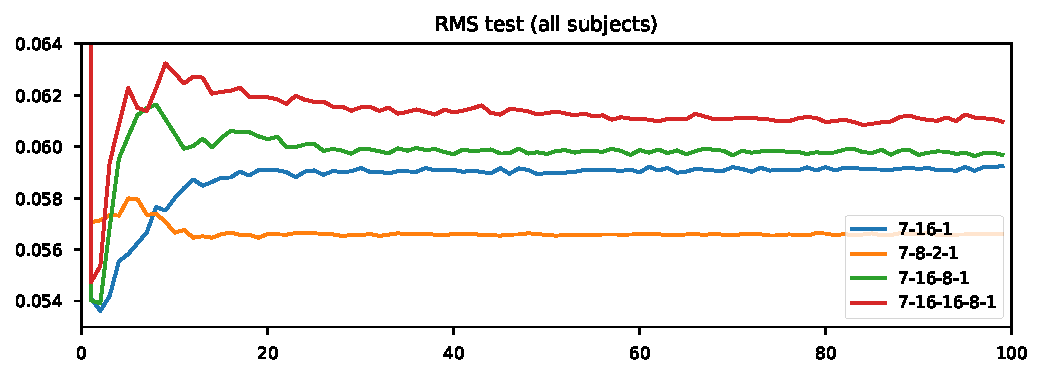
\includegraphics{rms-all-test-mlp-detail}
	\caption[Evolución del error en el conjunto de test durante el entrenamiento]{Visión en detalle de la evolución del error en el conjunto de test. Aunque no se ha considerado para determinar las arquitecturas, sí se ha recogido la información de la evolución del error en el conjunto de test debido a que nos ofrece puede ofrecer intuición de qué forma aprende la red. Por lo que podemos observar, para el problema en cuestión las redes más potentes tienden a sobre-entrenarse.}
	\label{fig:rms-all-test-mlp-detail}
\end{figure}

Una visión de detalle del ajuste de estas arquitecturas al conjunto de test se puede ver en la figura~\ref{fig:mlp-test-comparisons}, donde se muestra el perfil de aceleración del conjunto de test y los perfiles de aceleración de las redes entrenadas.

\begin{figure}
	\centering
	\subfloat[]{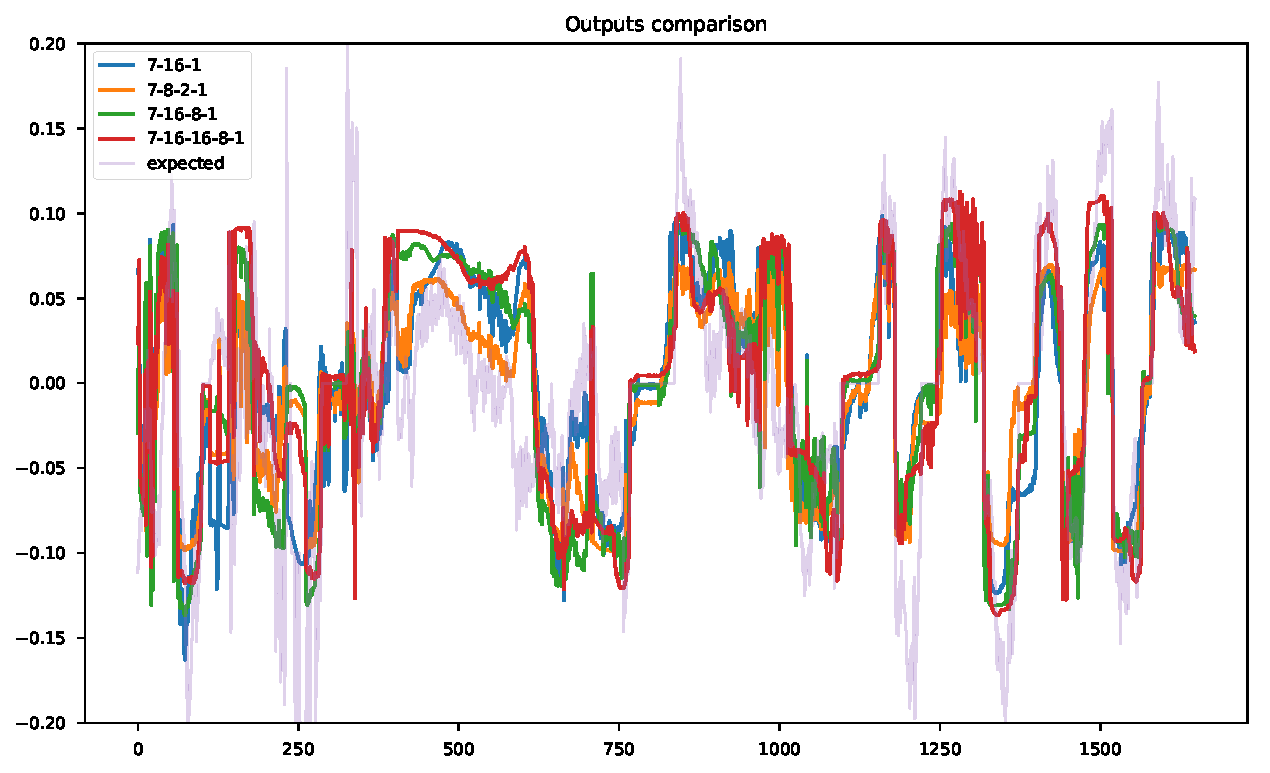
\includegraphics[width=.45\textwidth]{mlp-test-comparison}}\qquad
	\subfloat[]{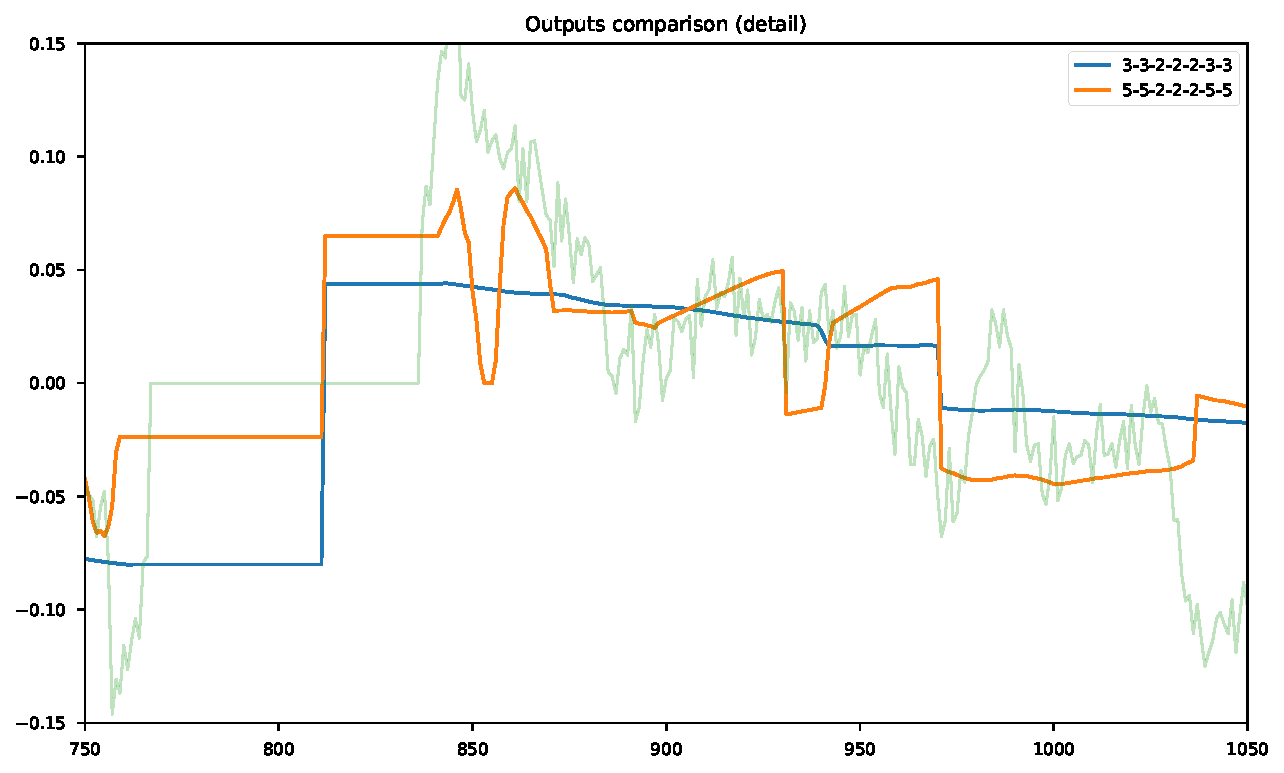
\includegraphics[width=.45\textwidth]{mlp-test-comparison-detail}}
	\caption[Comparación del perfil de aceleración real y el inferido por los modelos entrenados]{Comparación del perfil de aceleración real y el inferido por los modelos entrenados. En la visión general se puede observar, en transparente, el perfil real. A la derecha se amplía una pequeña sección del perfil para mostrar los diferentes ajustes de los modelos entrenados y cómo difieren del valor real.}
	\label{fig:mlp-test-comparisons}
\end{figure}

A la vista de los resultados, y dado que las arquitecturas se ajustan razonablemente bien, es razonable elegir el modelo $MLP_2$ debido a que es el que aparentemente mejor generaliza los comportamientos del conjunto de conductores.

\section{Comparación entre modelos}

Las mejores arquitecturas de ambos modelos han sido la $MLP_2$ para los \acp{mlp} y $FCS_x$ para los \acp{fcs}. Los errores y el perfil de aceleración para ambos modelos se muestran en la figura~\ref{fig:comparison-between-best-mlp-and-fcs-architecture}.

\begin{figure}
	\centering
	\subfloat[]{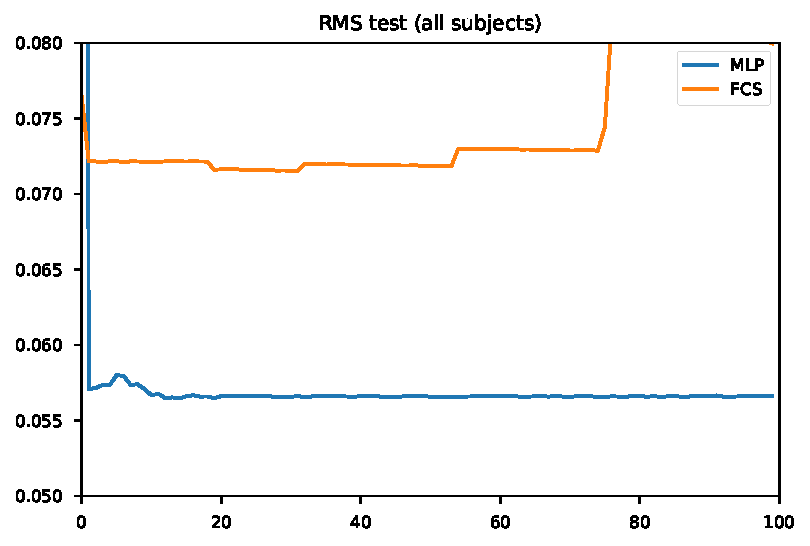
\includegraphics[width=.46\textwidth]{comparison-between-best-mlp-and-fcs-architecture-rms}}\qquad
	\subfloat[]{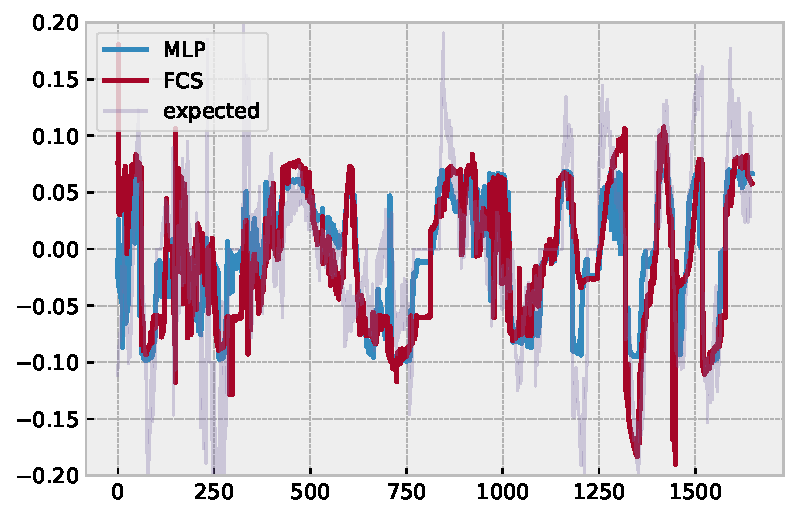
\includegraphics[width=.46\textwidth]{comparison-between-best-mlp-and-fcs-architecture-acceleration-profile}}
	\caption[Comparación entre los dos tipos de modelo longitudinal]{Comparación de la mejor arquitectura \ac{mlp} frente a la mejor arquitectura \ac{fcs}: (a) diferencia entre los errores cuadráticos medios de ambas arquitecturas y (b) perfiles de aceleración en el conjunto de test.}
	\label{fig:comparison-between-best-mlp-and-fcs-architecture}
\end{figure}

Aunque el modelo basado en \ac{fcs} arroja un error bajo en test y parece que tiende a ajustarse al perfil de aceleración, parece que el problema es suficientemente complejo como para no poder representarse como un simple controlador difuso.

Además, el error arrojado por el \ac{mlp} es sustancialmente menor y, por tanto, la arquitectura elegida para el modelo longitudinal será el \ac{mlp} $MLP_2$.